\documentclass[12pt, spanish]{report}
\usepackage[spanish, activeacute]{babel}
\usepackage[latin1]{inputenc}
\renewcommand{\baselinestretch}{1.3}
\usepackage{graphicx}

\begin{document}
\title{Universidad Sim�n Bol�var \\ Inteligencia II \\ Neurotic Pacman}
\author{
  Daniel Barreto - \#04-36723 \texttt{<daniel.barreto.n@gmail.com>} \\
  Edgar Henriquez - \#04-37105 \texttt{<edgarhenriquez@gmail.com>} \\
  Kristoffer Pantic - \#05-38675 \texttt{<kristoffer.pantic@gmail.com>}
}
\maketitle

\tableofcontents

\newpage

\chapter{Introducci�n}
\label{chap:intr}

\section{Definici�n del problema}
\label{sec:intr1}

\section{Pacman vs. Ms. Pacman}
\label{sec:intr2}


\chapter{Marco Te�rico: Investigaciones Previas}
\label{chap:mt}

\section{Simon M. Lucas: Evolving a Neural Network Location Evaluator
  to Play Ms. Pac-Man}
\label{sec:inv-prev}

\chapter{Implementaci�n}
\label{chap:impl}

\section{Herramientas usadas}
\label{sec:herr}

\section{Red Neural}
\label{sec:red}

\section{Algor�tmo gen�tico}
\label{sec:ag}

\section{Cambios y mejoras}
\label{sec:mejoras}

\subsection{Tasa de escalamiento de inputs}
\label{sec:escalamiento}

\subsection{Tasa de Neurotismo}
\label{sec:neurotismo}


\chapter{Experimentos y Resultados}
\label{chap:result}
En este cap�tulo se presentan los experimentos realizados para probar
la efectividad de los cambios realizados sobre nuestra implementaci�n
del agente \emph{NeuroticPacman}.

\section{Descripci�n de los experimentos}
\label{sec:desc-experimentos}
Tanto el algoritmo evolutivo de aprendizaje de \emph{NeuroticPacman}
como la red neural que sirve como su controlador, pueden ser ajustados
o configurados con ciertos par�metros de inter�s, los cuales son
mencionados a continuaci�n:

\subsection{Par�metros de configuraci�n para el algoritmo evolutivo de aprendizaje}
\begin{itemize}
\item Tama�o de la poblaci�n.
\item Porcentaje de la poblaci�n a ser mutada en una nueva generaci�n.
\item Cantidad de juegos utilizados para calcular el score average
  (fitness) de un individuo.
\end{itemize}

\subsection{Par�metros de configuraci�n para el controlador del agente}
\begin{itemize}
\item Cantidad de capas intermedias de la red neural.
\item Cantidad de neuronas en la(s) capa(s) intermedia(s).
\item \textbf{Tasa de escalamiento de inputs} (secci�n \ref{sec:escalamiento}).
\item \textbf{Tasa de Neurotismo} (secci�n \ref{sec:neurotismo}).
\end{itemize}

Para todos estos par�metros, la investigaci�n de
Lucas\cite{lucas:2005} cubre pruebas sobre la mejor configuraci�n de
todos los par�metros mencionados para el algoritmo evolutivo de
aprendizaje y para la cantidad de capas intermedias de la red neural y
la cantidad de neuronas en ellas. Lucas llega a sus mejores resultados
(Figura \ref{img:resultados-lucas}) usando la siguiente configuraci�n:

\begin{itemize}
\item Tama�o de la poblaci�n: \textbf{20}
\item Porcentaje de la poblaci�n a ser mutada en una nueva generaci�n:
  \textbf{50\%}
\item Cantidad de juegos utilizados para calcular el score average
  (fitness) de un individuo: \textbf{50}
\item Cantidad de capas intermedias de la red neural: \textbf{1}
\item Cantidad de neuronas en la capa intermedia: \textbf{20}
\end{itemize}

Los experimentos realizados en nuestro trabajo se basan completamente
en esta configuraci�n, y prueban los resultados de variar los �ltimos
dos par�metros mencionados: \textbf{Tasa de escalamiento de inputs} y
\textbf{Tasa de Neurotismo}.\\

Para estos dos par�metros, las variaciones tomadas fueron las
siguientes: La tasa de Neurotismo es variada entre los valores 1.5,
2.0 y 2.5 mientras que la tasa de escalamiento de inputs es variada
entre $\frac{1}{9.875}$, $\frac{1}{39.5}$, $1$ (sin tasa de
escalamiento).\\

Todas las corridas del algoritmo evolutivo se realizaron con 1000
generaciones, al igual que el trabajo original de
Lucas\ref{lucas:2005}, para poder establecer comparaciones con su
trabajo.

Por razones de tiempo, las pruebas realizadas sobre la tasa de
escalamiento entre los valores $\frac{1}{9.875}$ y $\frac{1}{39.5}$
fueron realizadas con �nicamente 100 generaciones, y no son reportadas
gr�ficamente, sin embargo los resultados mostraron que el uso del
valor $\frac{1}{9.875}$ tuvo mejores resultados.

\section{Pruebas principales}
\label{sec:pruebas-principales}

Los experimentos realizados buscan conseguir cual tasa de Neurotismo
hace que \emph{NeuroticPacman} tenga un mejor comportamiento usando la
tasa de escalamiento de inputs en $\frac{1}{9.875}$, y luego usando
dicha tasa, probamos deshabilitando la tasa de escalamiento.\\

Los resultados se encuentran detallados gr�ficamente a continuaci�n:

\newpage
\begin{center}
  \textbf{
    Tasa de Neurotismo: 1.5\\
    Tasa de escalamiento: 9.875 }
\end{center}
\begin{figure}[htp]
  \centering
  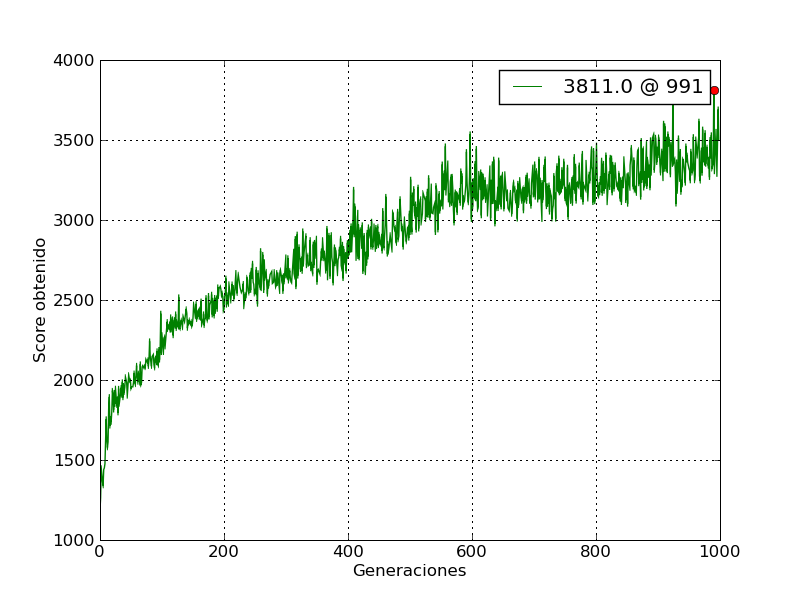
\includegraphics[scale=0.7]{logs/scores-7-12-2009-13-14-36.png}
  \caption{Mejor resultado obtenido: 3811.0 en la generaci�n 991}
\end{figure}

\newpage
\begin{center}
  \textbf{
    Tasa de Neurotismo: 2.0\\
    Tasa de escalamiento: 9.875 }
\end{center}
\begin{figure}[htp]
  \centering
  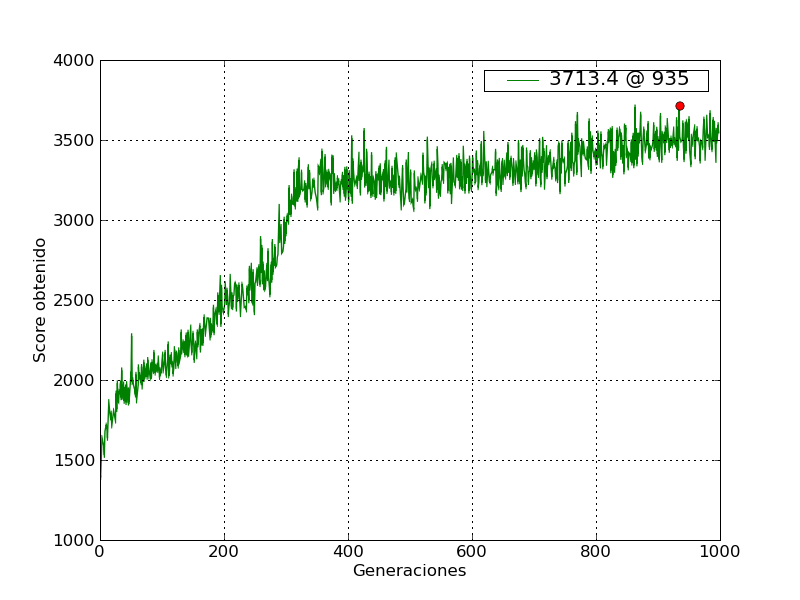
\includegraphics[scale=0.7]{logs/scores-6-12-2009-11-50-17.png}
  \caption{Mejor resultado obtenido: 3713.4 en la generaci�n 935}
\end{figure}

\newpage
\begin{center}
  \textbf{
    Tasa de Neurotismo: 2.5\\
    Tasa de escalamiento: 9.875 }
\end{center}
\begin{figure}[htp]
  \centering
  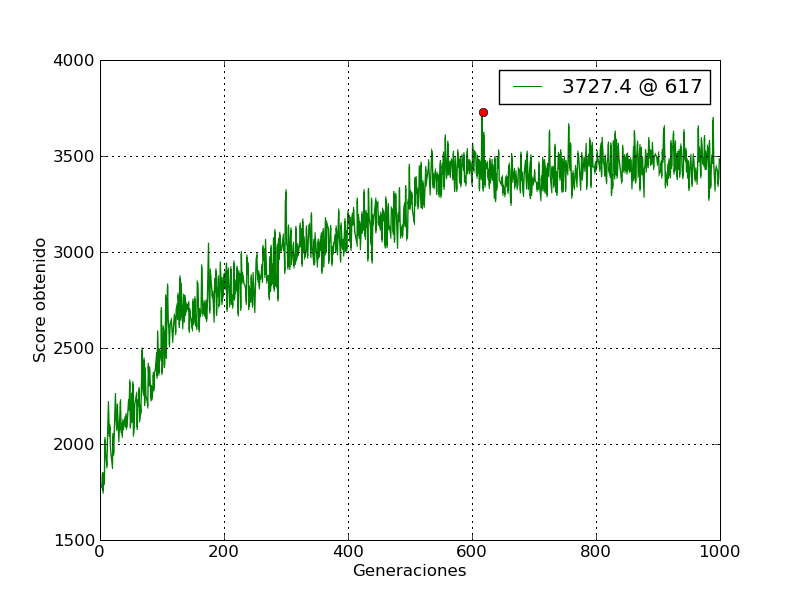
\includegraphics[scale=0.7]{logs/scores-6-12-2009-13-55-34.png}
  \caption{Mejor resultado obtenido: 3727.4 en la generaci�n 617}
\end{figure}

\newpage
\begin{center}
  \textbf{
    Tasa de Neurotismo: 1.5\\
    Tasa de escalamiento: 1 }
\end{center}
\begin{figure}[htp]
  \centering
  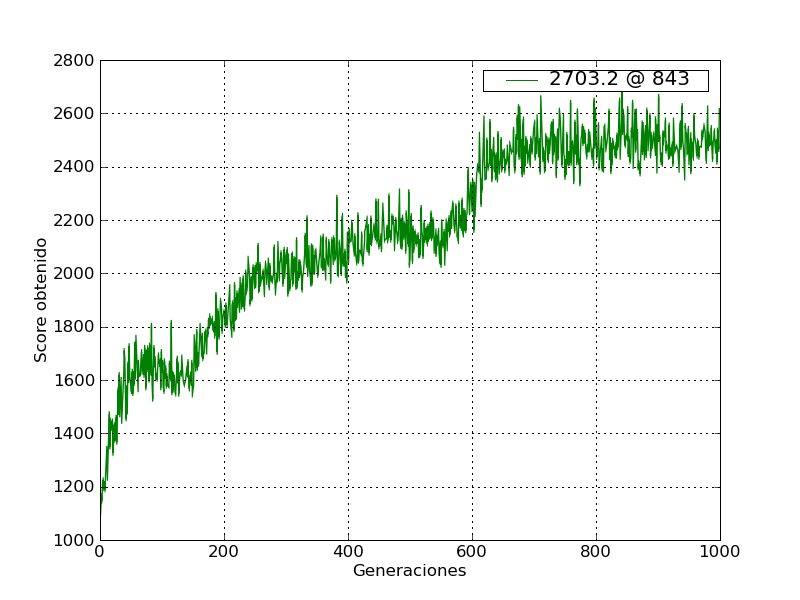
\includegraphics[scale=0.7]{logs/scores-7-12-2009-14-12-11.png}
  \caption{Mejor resultado obtenido: 2703.2 en la generaci�n 843}
\end{figure}

\newpage
\section{An�lisis de resultados}
\label{sec:analisis}

\bibliographystyle{plain}
\addcontentsline{toc}{chapter}{Bibliograf\'ia}
\bibliography{bibliography}

\end{document}